\documentclass[12pt,a4paper]{extreport}
\usepackage[l2tabu,orthodox]{nag}

\usepackage[left=15mm,right=15mm, top=20mm,bottom=20mm,bindingoffset=0cm]{geometry}

\usepackage{indentfirst}
\usepackage[labelsep=period]{caption}
\usepackage{amssymb,amsmath,amsthm}
\usepackage{fontspec}
\usepackage{float}
\usepackage{array}
\usepackage{listings}


\setmainfont[Ligatures=TeX]{STIX}
\newfontfamily{\cyrillicfont}[Ligatures=TeX]{STIX}
\setmonofont{Fira Mono}
\newfontfamily{\cyrillicfonttt}{Fira Mono}

\usepackage{polyglossia}
\setdefaultlanguage{russian}
\setotherlanguage{english}

\usepackage{subcaption}
\usepackage{graphicx}
\graphicspath{img/}
\DeclareGraphicsExtensions{.pdf,.png,.jpg}

\usepackage{color}
\definecolor{darkblue}{rgb}{0,0,.75}
\definecolor{darkred}{rgb}{.7,0,0}
\definecolor{darkgreen}{rgb}{0,.7,0}

\usepackage[normalem]{ulem}
\setlength{\marginparwidth}{2cm}
\usepackage[textwidth=4cm,textsize=tiny]{todonotes}
\newcommand{\fix}[2]{{\textcolor{red}{\uwave{#1}}\todo[fancyline]{#2}}}
\newcommand{\hl}[1]{{\textcolor{red}{#1}}}
\newcommand{\cmd}[1]{{\ttfamily{\textbackslash #1}}}

\newcommand{\vrb}[1]{\PVerb{#1}}
\newcommand{\vrbb}[1]{\texttt{\textbackslash}\PVerb{#1}}

\usepackage[
    draft = false,
    unicode = true,
    colorlinks = true,
    allcolors = blue,
    hyperfootnotes = true
]{hyperref}

\usepackage{tikz}
\usetikzlibrary{graphs, quotes}
\usepackage{relsize}
\usepackage{ytableau}

%\usepackage{titlesec}
%\titleformat{\subsection}{\normalfont\large\bfseries}{\thesubsection.}{\smallskip}{}
\renewcommand \thesection{\Roman{section}}
\renewcommand \thesubsection{\arabic{subsection}}

\theoremstyle{plain}
\newtheorem{theorem}{Теорема}
\newtheorem{lemma}{Лемма}
\newtheorem{proposition}{Утверждение}
\newtheorem{corollary}{Следствие}
\theoremstyle{definition}
\newtheorem{definition}{Определение}
\newtheorem{notation}{Обозначение}
\newtheorem{example}{Пример}
\newcommand\abs[1]{\left\lvert #1 \right\rvert}
\newcommand\ceil[1]{\left\lceil{#1}\right\rceil}
\newcommand\floor[1]{\left\lfloor{#1}\right\rfloor}
\newcommand{\divby}{\;\raisebox{-0.4ex}{\vdots}\;} 

\title{<<Самостоятельная работа по вычислению производных высших порядков>>}
\begin{document}
\maketitle
\pagebreak
\tableofcontents
\pagebreak
\section{Вступление}
В первом классе советской школы математика была не просто предметом, а боевым рубежом. Пока загнивающий Запад в детских садах изучал цвета радуги и делал поделки из макарон, наши первоклассники уже знали, что дифференцировать функции — это не прихоть, а вопрос государственной важности. С урока сразу на доске красовалось грозное: “ДЕРИВАТЫ — старшие братья численных рядов!”. Мелом, быстро и четко. 

Учительница Мария Ивановна, с легким прищуром и неотразимой верой в светлое будущее, объясняла суть производной на примере сбора картошки: “Если Ваня копает одну сотку за 10 минут, а Петя — за 5 минут, то чья производная выше?”. Кто не понимал, оставался после уроков считать частные производные по полям кукурузы.



Зато к концу первой четверти маленькие дифференциаторы могли находить скорость распространения слухов в очереди за колбасой, а на переменах спорили о втором законе Ньютона, пока взрослые стояли в очереди за учебниками. Такие времена, такой уровень. И если кто-то на вопрос “Чему равна производная синуса?” пытался сказать “Что такое синус?”, его тут же отправляли в третий класс — в народное хозяйство стране помощники нужны!\section{Вычисление}


Давайте продифференцируем данную легчайшую функцию.

\begin{dmath*}
f(x) = \arctg(x)
\end{dmath*}

Вычислим 1-ую производную:

\begin{dmath*}
f^{(1)}(x) = \frac{1}{1 + {x}^{2}}
\end{dmath*}
Давайте немного упростим данное выражение.


Получаем 1-ую производную:

\begin{dmath*}
f^{(1)}(x) = \frac{1}{1 + {x}^{2}}
\end{dmath*}

Вычислим 2-ую производную:

\begin{dmath*}
f^{(2)}(x) = \frac{0 \cdot 1 + {x}^{2} - 1 \cdot 0 + 2 \cdot {x}^{2 - 1}}{({1 + {x}^{2})}^{2}}
\end{dmath*}
Давайте немного упростим данное выражение.


Получаем 2-ую производную:

\begin{dmath*}
f^{(2)}(x) = \frac{2 \cdot x}{({1 + {x}^{2})}^{2}}
\end{dmath*}

Вычислим 3-ую производную:

\begin{dmath*}
f^{(3)}(x) = \frac{0 \cdot x + 2 \cdot 1 \cdot ({1 + {x}^{2})}^{2} - 2 \cdot x \cdot 2 \cdot 0 + 2 \cdot {x}^{2 - 1} \cdot ({1 + {x}^{2})}^{1}}{({({1 + {x}^{2})}^{2})}^{2}}
\end{dmath*}
Давайте немного упростим данное выражение.


Получаем 3-ую производную:

\begin{dmath*}
f^{(3)}(x) = \frac{2 \cdot ({1 + {x}^{2})}^{2} - 2 \cdot x \cdot 2 \cdot 2 \cdot x \cdot 1 + {x}^{2}}{({({1 + {x}^{2})}^{2})}^{2}}
\end{dmath*}

Вычислим 4-ую производную:

\begin{dmath*}
f^{(4)}(x) = \frac{0 \cdot ({1 + {x}^{2})}^{2} + 2 \cdot 2 \cdot 0 + 2 \cdot {x}^{2 - 1} \cdot ({1 + {x}^{2})}^{1} - 0 \cdot x + 2 \cdot 1 \cdot 2 \cdot 2 \cdot x \cdot 1 + {x}^{2} + 2 \cdot x \cdot 0 \cdot 2 \cdot x \cdot 1 + {x}^{2} + 2 \cdot 0 \cdot x + 2 \cdot 1 \cdot 1 + {x}^{2} + 2 \cdot x \cdot 0 + 2 \cdot {x}^{2 - 1} \cdot ({({1 + {x}^{2})}^{2})}^{2} - 2 \cdot ({1 + {x}^{2})}^{2} - 2 \cdot x \cdot 2 \cdot 2 \cdot x \cdot 1 + {x}^{2} \cdot 2 \cdot 2 \cdot 0 + 2 \cdot {x}^{2 - 1} \cdot ({1 + {x}^{2})}^{1} \cdot ({({1 + {x}^{2})}^{2})}^{1}}{({({({1 + {x}^{2})}^{2})}^{2})}^{2}}
\end{dmath*}
Давайте немного упростим данное выражение.


Получаем 4-ую производную:

\begin{dmath*}
f^{(4)}(x) = \frac{4 \cdot 2 \cdot x \cdot 1 + {x}^{2} - 4 \cdot 2 \cdot x \cdot 1 + {x}^{2} + 2 \cdot x \cdot 2 \cdot 2 \cdot 1 + {x}^{2} + 2 \cdot x \cdot 2 \cdot x \cdot ({({1 + {x}^{2})}^{2})}^{2} - 2 \cdot ({1 + {x}^{2})}^{2} - 2 \cdot x \cdot 2 \cdot 2 \cdot x \cdot 1 + {x}^{2} \cdot 2 \cdot 2 \cdot 2 \cdot x \cdot 1 + {x}^{2} \cdot ({1 + {x}^{2})}^{2}}{({({({1 + {x}^{2})}^{2})}^{2})}^{2}}
\end{dmath*}
\section{Заключение}
Наша функция и полученная производная:


\begin{dmath*}
f(x) = \arctg(x)
\end{dmath*}

\begin{dmath*}
f^{(4)}(x) = \frac{4 \cdot 2 \cdot x \cdot 1 + {x}^{2} - 4 \cdot 2 \cdot x \cdot 1 + {x}^{2} + 2 \cdot x \cdot 2 \cdot 2 \cdot 1 + {x}^{2} + 2 \cdot x \cdot 2 \cdot x \cdot ({({1 + {x}^{2})}^{2})}^{2} - 2 \cdot ({1 + {x}^{2})}^{2} - 2 \cdot x \cdot 2 \cdot 2 \cdot x \cdot 1 + {x}^{2} \cdot 2 \cdot 2 \cdot 2 \cdot x \cdot 1 + {x}^{2} \cdot ({1 + {x}^{2})}^{2}}{({({({1 + {x}^{2})}^{2})}^{2})}^{2}}
\end{dmath*}


Несложно заметить, что графики выглядят так:

\begin{minipage}{0.45\textwidth}
\centering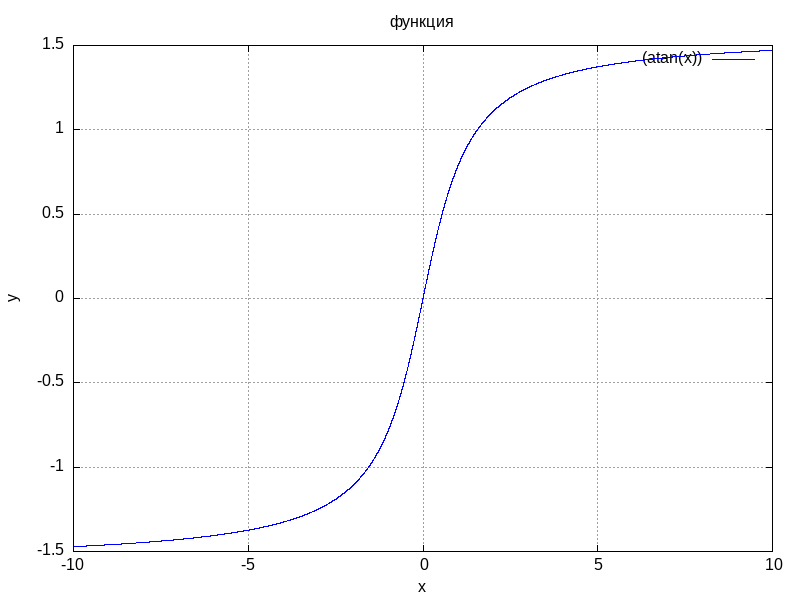
\includegraphics[width=\linewidth]{out/orig_plot.png}\end{minipage}
\hfill
\begin{minipage}{0.45\textwidth}
\centering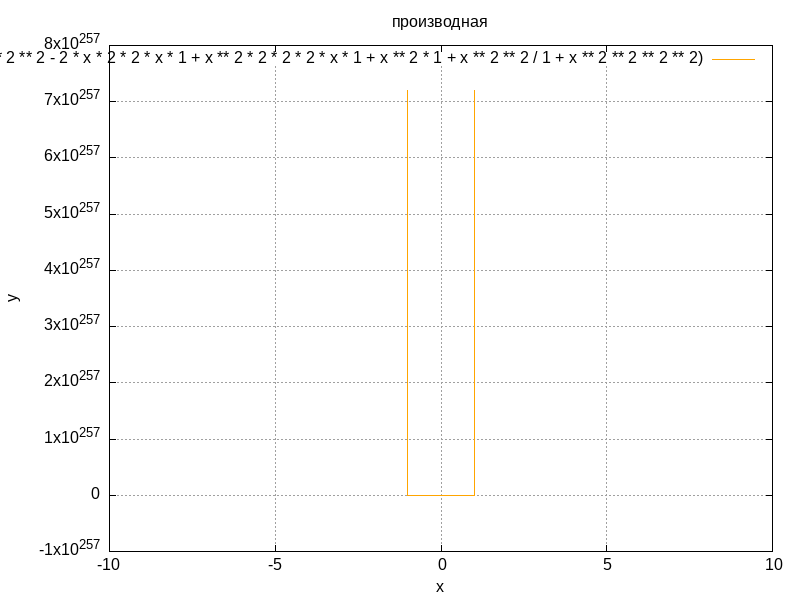
\includegraphics[width=\linewidth]{out/optimized_plot.png}\end{minipage}
\end{document}
